\setlength{\tabcolsep}{6pt}
\renewcommand{\arraystretch}{-1}

\begin{tabular}{
  >{\centering\arraybackslash}p{3.5cm}|   % nouvelle colonne regroupement
  p{7cm}
  >{\centering\arraybackslash}p{3cm}
  >{\centering\arraybackslash}p{1.8cm}
  >{\centering\arraybackslash}p{1.8cm}
  >{\centering\arraybackslash}p{1.8cm}
  >{\centering\arraybackslash}p{1.8cm}
  }
  \rowcolor{black!10}
  \textbf{Tendance famille IA} & \textbf{Catégorie de travaux}                                         & \textbf{C1 Autonomie}              & \textbf{C2 Perf.}                   & \textbf{C3 Adapt.}                  & \textbf{C4 Contrôle}                & \textbf{C5 Explic.} \\
  \hline

  % ------------------------- SYMBOLIQUE -------------------------
  \multirow{3}{*}[-0.35cm]{\vspace{0.9cm}\textbf{$\sim$ \textit{Symbolique}}}
                               & {\vspace{0.25cm}\textbf{Systèmes experts $\sim$ SMA de Cyberdéfense}}

    {\tiny \begin{spacing}{0.8}
               \textbf{hierarchies \& essaims}~\parencite{holloway2009self,lamont2009military,holloway2019self}, \textbf{méthodes évolutionnaires}~\parencite{akandwanaho2018generic,carvalho2011evolutionary}, \textbf{architectures réactives}~\parencite{de2017distributed}, \textbf{bio-inspirés}~\parencite{haack2011ant}, \textbf{cadres cyber-physiques}~\parencite{demir2021adaptive}, \textbf{CIDS}~\parencite{vasilomanolakis2015taxonomy}
             \end{spacing}}






                               & {\vspace{0.65cm}\xmark~--~$\sim$}                                     & {\vspace{0.65cm} $\sim$ }          & {\vspace{0.65cm} $\sim$ }           & {\vspace{0.65cm} \cmark }           & {\vspace{0.65cm} \cmark }                                 \\

                               & \textbf{Modélisation d’environnement}
  {\tiny \begin{spacing}{0.8}
             \textbf{modèles formels (POMDP, Dec-POMDP, POSG)}~\parencite{Oliehoek2016, Beynier2013}, \textbf{théorie jeux}~\parencite{MPanfili2018,AAttiah2018,CXiaolin2008}, \textbf{graphes attaque}~\parencite{CPhilips1998}, \textbf{arbres attaque-défense}~\parencite{BKordy2010}, \textbf{réseaux Petri}~\parencite{SYamaguchi2020}
           \end{spacing}}


                               & {\vspace{0.2cm} \xmark }                                              & {\vspace{0.2cm} $\sim$    }        & {\vspace{0.2cm} $\sim$ }            & {\vspace{0.2cm} \cmark }            & {\vspace{0.2cm} \cmark }                                  \\

                               & \textbf{Cadres de conception SMA}
  {\tiny \begin{spacing}{0.8}
             \textbf{simulation réseaux}~\parencite{Standen2021, janisch2023nasimemu}, \textbf{frameworks entraînement}~\parencite{hammar_stadler_noms_22, CROND}, \textbf{plateformes expérimentations}~\parencite{Niculae2018, cyberbattlesim}
           \end{spacing}}
                               & {\vspace{0.12cm}\cmark }                                              & {\vspace{0.12cm} \cmark  }         & {\vspace{0.12cm} $\sim$~--~\cmark } & {\vspace{0.12cm} \xmark }           & {\vspace{0.12cm} \xmark~--~$\sim$ }                       \\

  \vspace{-4.45cm}

  \multirow{1}{*}{
    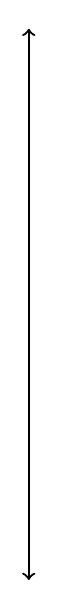
\begin{tikzpicture}
      \draw[<->, thick] (0,1)--(0,8);
      \vspace{1cm}
    \end{tikzpicture}
  }



  % ---------------------- CONNEXIONNISTE ------------------------
  \multirow{3}{*}{\vspace{-14.3cm}\textbf{$\sim$ \textit{Connexionniste}}}
  \vspace{-0.35cm}
                               & \textbf{Maintien cohérence simulation/réel}

  {\tiny \begin{spacing}{0.8}
             \textbf{Robust RL}~\parencite{pinto2017robust}, \textbf{Sim2Real}~\parencite{tobin2017domain,ganin2016domain}, \textbf{calibration dynamique}~\parencite{deisenroth2011pilco}
           \end{spacing}}

                               & {\vspace{-0.12cm}$\sim$~--~\cmark }                                   & {\vspace{-0.12cm}n/a }             & {\vspace{-0.12cm} \cmark }          & {\vspace{-0.12cm} $\sim$ }          & {\vspace{-0.12cm} $\sim$ }                                \\

                               & \textbf{MARL \& contraintes organisationnelles}

  {\tiny \begin{spacing}{0.8}
             \textbf{CPO}~\parencite{achiam2017constrained}, \textbf{Deep Constrained Q-Learning}~\parencite{kalweit2020deep}, \textbf{Safe RL}~\parencite{garcia2015comprehensive}, \textbf{Deep TAMER}~\parencite{warnell2018deep}, \textbf{reward shaping}~\parencite{ng1999policy}, \textbf{shielding}~\parencite{amodei2016concrete}
           \end{spacing}}

                               & {\vspace{0.06cm}\xmark~--~$\sim$ }                                    & {\vspace{0.06cm}$\sim$~--~\cmark } & {\vspace{0.06cm} $\sim$ }           & {\vspace{0.06cm} \cmark }           & {\vspace{0.06cm} $\sim$~--~\cmark }                       \\

                               & \textbf{Extraction organisationnelle émergente}
  {\tiny \begin{spacing}{0.8}
             \textbf{extraction arbres}~\parencite{milani2022maviper,zhang2024advancing}, \textbf{décompositions valeur}~\parencite{Sunehag2018,Tabish2018}, \textbf{attributions Shapley}~\parencite{heuillet2021collective}, \textbf{inférence rôles émergents}~\parencite{Wang2020}
           \end{spacing}}

                               & {\vspace{0.06cm} \xmark~--~$\sim$ }                                   & {\vspace{0.06cm} $\sim$  }         & {\vspace{0.06cm} $\sim$ }           & {\vspace{0.06cm} \xmark~--~$\sim$ } & {\vspace{0.06cm} \cmark }                                 \\[0.001cm]
  \hline
\end{tabular}
